\section{The Latitude Blockchain}\label{sec:design}

In this section, we present a high-level design of the Latitude blockchain. The full-version of this whitepaper shall
contain a very detailed design of each component. We start with an overview of the key design principles that will guide
the rest of the design for the Latitude Blockchain. Its important to note here that for implementation purposes, it
might be possible to use an existing core blockchain for the underlying functionalities and build Latitude as a layer on
top. We shall make these determinations in the full-version of the whitepaper.

\subsection{Overview of design principles}

The purpose of the Latitude blockchain is to become the best platform in the world for decentralized applications for
the Transportation Industry. Specifically, this boils down to constructs in the blockchain that can handle spatial,
mapping, traffic, driving data including data relating to other modalities of transport (bike sharing, walking, even air
routes later on). Figure XXX presents the architecture of the Latitude blockchain in terms of the core technological
innovations that will be built into it.

\begin{figure}[t]
    \centering
    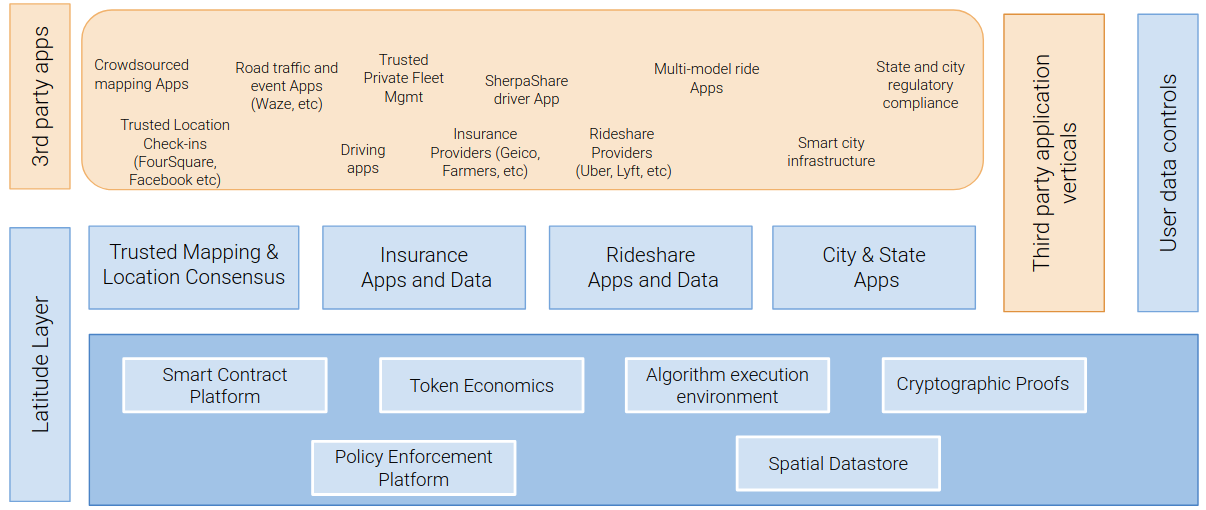
\includegraphics[width=0.90\textwidth]{latarch.png}
  \caption{Architecture of the Latitude Blockchain and associated platform ecosystem.}
    \label{fig:lat-arch}
\end{figure}


Datastore
 - Optimized for Geographic, Geo-spatial data.
 - Location, Mapping data and computation.
 - Ability to Store, index, query and build smart contracts optimized for such data.
 - Support for various spatial indexes.
 - Location heatmaps.
 - Indexing road and driving data.
 - Primitives for storing driving data for autonomous vehicles

Cryptographic primitives for:
 - Security and privacy of data.
 - Anonymity guarantees using cryptographic set operations.
 - Enforcement of privacy when sharing data.
 - Sharing of “computation” instead of data when possible.
 - For eg: Sharing of DriverScore using a vetted algorithm.
 - Sharing proximity to a landmark instead of lat/lng.
 - Ability to find bad actors.
 - Detect privacy, anonymity and security violations.


Smart contract system for Transportation applications.
 - Ability to convert “policies” such as GDPR into smart contract code.
 - Example, self destruct data after a time period.
 - Sandboxed trusted execution environment:
 - For algorithms:
   - DriverScore, Location heatmaps, Statistics.
   - Enforcing or verifying privacy and other govt policies/regulations.

Cryptographic proofs for applications:
 - Proof of Location. 
 - Proof of ride. 
 - Proof of mapping 
      (road/landmark exists or does not exist).
 - Proof of driver score 
 - Open, trusted, understood driver score computation algorithms.
 - Cryptographic proofs can be shared among entities, safely, securely.


Cryptoeconomics and Governance:
 - Crypto-incentives for honest operation.
 - Penalties for malicious intent.
 - Governance based on consensus and roles using a council.
 - Council members elected using voting, stake and established trust.
 - Some council members can have restricted access.
 - Eg: US govt can have voting rights on US data/users, etc.

User incentives:
 - Users have full control over their data and computation.
 - Users can issue or request proofs to carry over to other applications.
 - User’s have incentive to share data, participate in improving the common denominator.
 - Malicious intent, Byzantine behavior.
   - Can be detected using a combination of consensus and incentives.
   - Best interest of users to act honestly by design.

\subsection{Blockchain Architecture}



Performance:
- Transaction speed. Data throughput. Storage capabilities.
